\documentclass[10pt, twocolumn]{article}

\usepackage{fullpage}
\usepackage{amsmath}
\usepackage{amssymb}
\usepackage{listings}
\usepackage{anyfontsize}
\usepackage{subcaption}
\usepackage{graphicx}
\usepackage{titling}
\usepackage{array}
\usepackage{authblk}

\setlength{\droptitle}{-4em}   % This is your set screw

\title{Latent Predicate Networks: Concept Learning with Probabilistic Context-Sensitive Grammars}
\author{Eyal Dechter (edechter)}
\author{Joshua Rule (rule)}
\author{Joshua B. Tenenbaum (jbt)}
\affil{Department of Brain and Cognitive Sciences, MIT (mit.edu)}

\renewcommand\Authands{ and }
\date{}

\begin{document}
\vspace{-10cm}
\maketitle
\vspace{-4em}

{\small For humans, learning abstract concepts and learning language
  go hand in hand: we acquire abstract knowledge primarily through
  linguistic experience, and acquiring abstract concepts is a crucial
  step in learning the meanings of linguistic expressions. Number
  knowledge is a case in point: we largely acquire concepts such as
  seventy-three through linguistic means, and we can only know what
  the sentence ``Seventy-three is more than twice as big as
  thirty-one" means if we can grasp the meanings of its component
  number words. How do we begin to solve this problem? One approach is
  to estimate the distribution from which sentences are drawn, and, in
  doing so, infer the latent concepts and relationships that best
  explain those sentences. We present early work on a learning
  framework called Latent Predicate Networks (LPNs) which learns
  concepts by inferring the parameters of probabilistic
  context-sensitive grammars over sentences.  We show that for a small
  fragment of sentences expressing relationships between English
  number words, we can use hierarchical Bayesian inference to learn
  LPNs that can answer simple queries about previously unseen
  relationships within this domain. These generalizations demonstrate
  LPNs' promise as a tool for learning and representing conceptual
  knowledge in language.}

\section{Introduction}

Although concept learning and language acquisition have typically been
treated as distinct problems in AI, linguistics and cognitive
development, they are strongly coupled for a child learning to
understand language. More generally, people learn many abstract
concepts primarily through language even though understanding language
depends on understanding the underlying concepts. Research in concept
learning is often focused on concepts grounded in perceptual features,
and while it is almost certainly true that many concepts are learned
via generalization from concrete examples, some concepts cannot be
learned this way.

Number concepts are a good example: children do not learn about the
meaning of ``seventy five'' by seeing examples of seventy five things;
they do not know that ``seventy five'' is more than ``twenty five''
because of their perceptual experiences of these quantities. Rather,
children learn the meaning of ``seventy five'' (or ``a billion and
five'') by noticing how number words are used in language, in counting
sequences, in arithmetic excercises, {\it etc}. Other good examples of such
abstract concepts are kinship and social relations ({\it e.g.} ``my father
in law's grandmother''), temporal relations (``the day after last
Thanksgiving.''), and spatial relations (``above and just to the left
of'').

Such abstract systems of concepts share many of the properties of
language syntax: there is an unbounded set of concepts, they derive
their meanings via composition, and, although people only ever say,
hear, or read about a small number of them, they are able to reason
correctly about any them. There seems to be a grammar to these
concepts, and grasping this grammar is critical to understanding their
meanings and how to use them. This motivates our approach here, which
is to apply the tools of probabilistic grammars more familiar from
studies of syntax to the problem of concept aquisition.

Doing so requires overcoming some technical barriers.

First, whereas context-free grammars are suitable for describing large
swaths of language syntax, the grammars of concepts are not
context-free. To address this, we use Range Concatentation Grammars, a
context-sensitive grammar formalism -- one of several developed within
linguistics -- and extend this formalism to a probabilistic model of
sentences. 

Second, the categories of syntax -- the nonterminals of the grammar --
are often assumed to be known to children innately and given to
automated learners by human experts. The categories that underlie
conceptual knowledge, on the other hand, are far more numerous, vary
from domain to domain, and are unlikely to be known to the
learner. This motivates our use of latent predicates that, through
learning, assume the role of a domain's underlying concepts (in the
number domain, these might correspond to the concepts of
successorship, order of magnitude, magnitude comparison, exact
vs. approximate, {\it etc}.).

Finally, inducing probabilistic context-sensitive grammars with latent
predicates threatens to be intractable: our goal is to find a
middle ground between expressivity and tractability. Using
PRISM~\cite{DBLP:journals/jair/SatoK01} -- a probabilistic logic programming system that naturally
implements efficient dynamic programming algorithms for our models --
we are able to explore which domains and which grammar architectures
are a good fit for this grammar-based approach.

The rest of this paper describes early work on this approach. First,
we present Latent Predicate Networks (LPNs), our probabilistic model
of concept learning. Then, we describe our approach to inference and
its implementation in PRISM. Finally, we present preliminary
experimental results in the domain of number concept learning that
demonstrate the promise of this approach.

% people learn about many
% abstract concepts primarily through language and, conversely, these
% abstract concepts are critical to understanding language. Consider a
% child learning the meaning of the number words: the meaning of the
% ``seventy five'' is learned not by seeing collections of seventy five
% things but rather by understanding how ``seventy five'' is used in the
% various sentences, counting sequences, arithmetic excercises, etc.

% As Claude Shannon demonstrated with his
% guessing game experiment in 1950~\cite{Shannon1950}, an adult English
% speaker's understanding of her language and her world is such that the
% entropy of a character in English text is slightly more than one
% bit. Plausibly, any machine learning system able to predict natural
% language text with such accuracy will have learned much about the
% concepts expressed in that text. This intuition motivates us to invert
% Shannon's experiment and learn linguistic concepts by learning a
% probabilistic generative model for natural language.

% Probabilistic Context Free Grammars (PCFGs) are popular and much
% studied generative models for natural language
% syntax~\cite{Someone}. While debate continues about their ability to
% express the syntax of natural language, it is agreed that they cannot
% express dependencies between words that depend upon each other for
% their meaning. Consider an example from the domain of sentences
% addressed in this paper: ``after twenty eight comes twenty nine.''
% The second ``twenty'' depends on the first ``twenty'' and the
% ``eight'', and the ``nine'' depends on the ``eight''. This pattern is
% a clear example of the \emph{cross-serial dependencies} which
% context-free grammars cannot support.

% Our approach, then, will be to explore the use of probabilistic
% context \emph{sensitive} grammars for modeling natural language,
% extending the tools of hierarchical grammar induction~\cite{SOMEONE} from
% context-free grammars to ones that can express not only syntactic
% relationships but semantic ones as well. In the place of latent
% syntactic categories, we will refer to latent predicates -- relations
% between sentence components -- that, when learned, should correspond
% to the concepts that underlie sentence semantics.

% To explore this approach, we introduce a probabilisitic model called a
% Latent Predicate Network (LPN), and describe an inference procedure to
% learn its parameters using the probabilistic logic programming
% language PRISM. Finally, we study its performance when trained on
% sentences describing the relationships between numbers.

\section{Latent Predicate Networks}

\begin{figure}[t]
		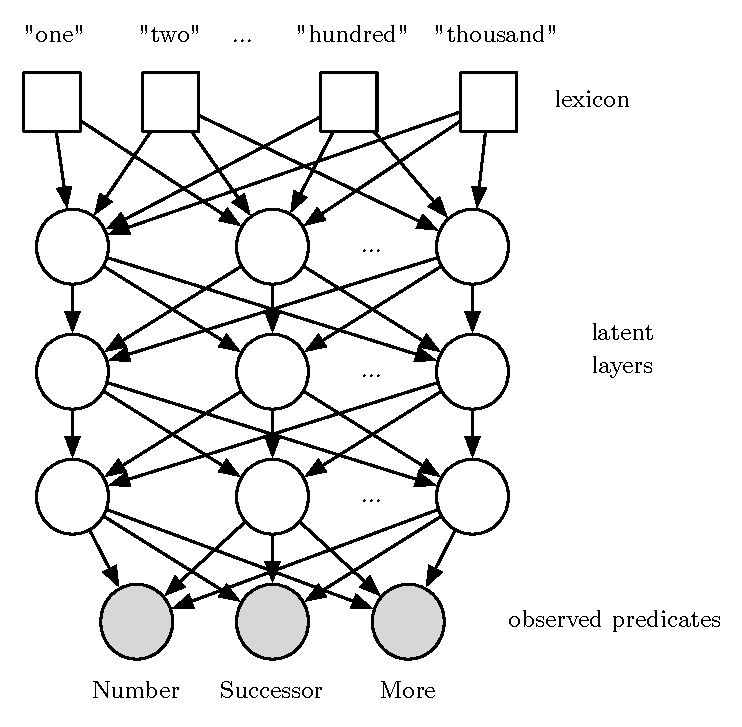
\includegraphics[width=\linewidth]{lpn/lpn.pdf}
		\caption{A schematic LPN.}
		\label{fig:architecture}
\end{figure}

An LPN is a hierarchical Bayesian model of strings
extending the Hierarchical Dirichlet PCFG model (HD-PCFG) to
Probabilistic Range Concatenation Grammars (PRCGs). 

\subsection{Probabilistic Range Concatentation Grammars}
Range Concatenation Grammars (RCGs) are a class of string grammars
that represent all and only those languages that can be parsed in time
polynomial in the length of the target
string~\cite{boullier2005range}. An RCG $G=(N, T, V, P, S)$ is a
5-tuple where $N$ is a finite set of predicate symbols, $T$ is a set
of terminal symbols, $V$ is a set of variable symbols, P is a finite
set of $M \geq 0$ clauses of the form $\psi_0 \rightarrow \psi_1 \dots
\psi_M$, and $S \in N$ is the \emph{axiom}. Each $\psi_m$ is a term of
the form $A(\alpha_1, \dots, \alpha_{\mathcal{A}(A)}$, where $A \in
N$, $\mathcal{A}(A)$ is the arity of $A$, and each $\alpha_i \in (T
\cup V)^*$ is an argument of $\psi_m$. We call the left hand side term
of any clause the \emph{head} of that clause and its predicate symbol
is the \emph{head predicate}.

%% \textbf{Example:} The following is an RCG for the 3-copy language
%% $\{www | w \in \{a, b\}^*\}$:
%% \begin{alignat*}{3}
%% &S(XYZ) &&\rightarrow A(X, Y, Z)\\
%% &A(aX, aY, aZ) &&\rightarrow A(X, Y, Z)\\
%% &A(bX, bY, bZ) &&\rightarrow A(X, Y, Z)\\
%% &A(\epsilon, \epsilon, \epsilon) &&\rightarrow 
%% \end{alignat*}

A string $x$ is in the language defined by an RCG if one can
\emph{derive} $S(x)$. A derivation is a sequence of rewrite steps in
which substrings of the left hand side argument string are bound to
the variables of the head of some clause, thus determining the
arguments in the clause body. If a clause has no body terms, then its
head is derived; otherwise, its head is derived if its body clauses
are derived.\footnote{This description of the language of an RCG
  technically only holds for \emph{non-combinatory} RCGs, in which the
  arguments of body terms can only contain single variables. Since any
  \emph{combinatory} RCG can be converted into a non-combinatory RCG
  and we only consider non-combinatory RCGs here, this description
  suffices.}

We extend RCGs to PRCGs by annotating each clause $C_k \in P$ with
probabilities $p_k$ such that for all predicates ${A \in N, \,
  \sum_{k:head(C_k)=A} p_k = 1}$. An PRCG defines a distribution over
strings $x$ by sampling from derivations of $S(x)$ according to the
product of probabilities of clauses used in that derivation. This is a
well defined distribution as long as no probability mass is placed on
derivations of infinite length; in this paper, we only consider PRCGs
with derivations of finite length, so we need not worry about this
requirement. See Figure \ref{fig:grammar} for an example of the context-sensitive 2-copy language $\{ww\,|w \in \{a,b\}^+\}$ as a PRCG.

\subsection{Generic Architecture}

An LPN is an PRCG with the following generic architecture: the
\emph{axiom} of an LPN is a unary predicate $S$, and it has $K$
densely connected binary predicates $\{A_k\}_{k=1}^K$ (Figure
\ref{fig:architecture}). For each latent predicate $A_k$, we define
rules such that $A_k(w_a,w_b)$ is true for each possible pair of
terminals, $w_a,w_b \in T$. $T$ may include the empty string $\epsilon$, but we
do not allow latent predicates of the form $A_k(\epsilon, \epsilon)$:
see Section~\ref{sec:implementation}. We also define rules such that
$A_k(XY,UV)$ is true for each possible pair of predicates, $A_i,A_j$,
and every possible ordering of the variables $X,Y,U$ and $V$ across
$A_i$ and $A_j$. Finally, we define $S(XY)$ to be the concatenation of
the two arguments of $A_1(X,Y)$.
 
% Now we can describe the model we introduce here, the Latent Concept
% Grammar (LCG). We introduce the LCG as a machine learning model to
% learn a distribution over instances of relations over strings. Unlike
% a PRCG, which places a distribution over terms RCGs consist of a set
% of rewrite rules, called clauses, each of which takes a termwhich
% operate on a set of terms (predicates applied to arguments) to produce
% new terms. Each rewrite rule is of the form:

% The vast majority of the models of concept acquisition that have been
% proposed in the artificial intelligence, machine learning and
% cognitive science literatures cannot represent the conceptual systems
% that even young children learn. Take, for example, the school-age
% child's knowledge of number. This child knows that there is no largest
% number; that ``one million forty three'' and ``8439''denote numbers
% but that ``one million forty billion'' and ``a82bd'' do not; that no
% two cardinalities refer to the same quantity but that some number
% words refer to the same cardinalities (e.g. ``two thousand'' and
% ``twenty-one hundred''). Moreover, the child knows how to guage the
% approximate number of elements in a collection and how to count this
% number exactly. In short, the child's knowledge of number consists of
% a complex system of concepts over an unbounded set of entities
% (i.e. the numbers). 

% Children are not born with this kind of knowledge, and, since number
% is a relatively recent cultural invention, nor is it likely that
% children possess innate domain specific background knowledge that
% makes it easier to acquire. Children only ever see a tiny fraction of
% all the numbers they can reason about and this evidence is biased,
% noisy, and can be unreliable. 

% A fundamental challenge for cognitive science -- and for any field
% interested in understanding human-like concept acquisition -- is to
% provide a theory of how such complex systems of concepts can be
% learned from sparse and noisy data.

% People are able to learn about complex systems of related
% concepts from small amounts of noisy data. A compelling approach to
% understanding such learning is to frame it as Bayesian inference over
% probabilistic knowledge bases. Advances in context free grammar
% induction in the past couple of decades can be seen as an instance of
% this approach, in which

% Our goal is to understand how children can obtain semantic knowledge
% about a system of concepts from the structure of relavent perceptual
% stimuli. How does a child learn that prefixing ``great-'' corresponds
% to adding an additional generation in kinship relationships? How does
% a child learn that ``just before'' is after ``a while before'' which
% is before ``a while after''? How does a child learn that if
% Figure~\ref{pairOfApples} is ``a pair of apples'' then
% Figure~\ref{singleApple} is a single apple? 

% Our proposal is that some interesting fragments of human conceptual
% knowledge can be represented as structured relations between
% linguistic tokens and other perceptual inputs; that the rules that
% define these relations implicitly define the concepts that are
% learned; and that these rules can be learned using the tools of
% hierarchical Bayesian inference. 

% For example, the concept TWENTY SEVEN is defined as the collection of
% representations ``27'', ``twenty seven'', ``3 times 9,'' along with a
% system of symbolic rules that translate among these representations
% and facilitate answered various queries. According to our hypothesis,
% the difference between TWENTY EIGHT and TWENTY SEVEN is not that they
% are represented in the mind by distinct mental symbols but rather that
% the rules that operate on their various representations treat them in
% systematically different ways.

% This view implies that an attempt to construct a computational account
% of concept learning in humans needs to ground out that learning in the
% relavent perceptual stimuli. 

% Contribution:
% \begin{itemize}
% \item We present Generate Rewrite Systems (GRS) -- a formalism that borrows
%   heavily from Linear Context-Free Rewriting Systems (CITE)
% \item We show how GRS, though restricted in representational capactiy,
%   can capture substantial cognitively plausible first-order conceptual knowledge 
% \item We propose a heirarchical Bayesian model for GRS that provides a coherent framework in which a GRS can be learned given evidence
% \item We show how GRS can be transformed into PRISM programs and learned within that probabilstic logic programming system
% \item We provide computational experiments that provide evidence that
%   our model can provide an account of some kinds of complex conceptual
%   knowledge can be inferred from noisy and sparse data
% \end{itemize}

% \section{The Model}

% Suppose we are given some positive instances $y_1, \dots,
% y_M$ of relations $R_1, \dots, R_N$. Our model assumes that each
% positive instance $y_m=R_n(\vec(x_m))$ is sampled i.i.d from a latent
% stochastic grammar (LSG), $\mathcal{K}$. $\mathcal{K}$ consists of
% some fixed number $K$ of clauses (i.e. rules) $C_1, \dots, C_K$ over
% the $N$ observable relations plus a fixed number of $H$ hidden
% relations $T_1, \dots, T_H$. The \emph{architecture} of the model is
% the exact specification of the parameters $K$ and $H$ and the clauses
% $\mathcal{C}$. To each clause $C_i$ is associated a positive real
% weights $\theta_i$.

% The clauses of $\mathcal{K}$ are Horn clauses in a first order logic
% with string concatenation. We will use PROLOG notation, in which lower
% case letters are predicates and constants and uppercase letters are
% variables. If two symbols are adjacent it means that the corresponding
% strings are concatenated. For example, the following would is a valid
% clause: $a(XY, XV) \leftarrow b(X, UV), a(X, X)$. In this rule $a$ and
% $b$ are relations with arity two.

% Let $C_1, \dots, C_{N(R)} = C(R)$ be the set of clauses whose head is
% relation $R$ and let $\Theta_R$ be the set of corresponding
% weights. Let $p_R(C_n) \sim \text{Discrete}(\Theta_R)$; that is, $p_R$
% is a distribution over the clauses headed by $R$, such that each
% clauses is sampled in proportion to its weight parameter.

% A positive instance of this relation is sampled from $\mathcal{K}$ by
% arbitrarily (i.e. uniformly at random) choosing a relation $R$ and
% instantiating that relation by sampling a clause from $p_R$. Recursing
% on this procedure for every atom in the body of this clause binds the
% variables in the clause's head. 

% Given this assumed generative process for the evidence, learning a
% program involves inferring the parameter $\theta$ given a prior
% probability distribution over their values. We place an independent
% Dirichlet distribution over the parameters of every relation. This is
% a natural choice that enables us to promote sparse programs, i.e.,
% programs in which most of the mass is placed on a small number of
% predicates and rules.

\subsection{Learning Model}

Given a collection of predicates, $\{A_k\}_{k=1}^{K}$, and a
distribution over clauses, $\{\vec{w}_{A_k}\}$, the learning task is
to model a set of utterances, $\{x_j\}_{j=1}^{J}$, as being generated
according to the following distribution:

\begin{align*}
  \vec{w}_{A_k} &\sim Dir(\vec{\alpha}_{A_k})\\
  x_j &\underset{iid}{\sim} p_{\text{\textsc{prcg}}}(S(x_j)\,|\,\{w_{A_k}\})
\end{align*}

\[ p(\{\vec{w}_{A_k}\}\,|\, \vec{x}, \{\vec{\alpha}_{A_k}\}) \propto\]\[ \prod_j
p_{\text{\textsc{prcg}}}(x_j|\{\vec{w}_{A_k}\}) \prod_{A_k} p_{\text{\textsc{dir}}}(\vec{w}_{A_k}\,|\,\vec{\alpha}_{A_k}) \]

In words, the weights of clauses sharing head predicate $A_k$ are drawn from a Dirichlet distribution defined by $\vec{\alpha}_{A_k}$. Sentences $x_j$ are then drawn from the resultant PRCG.

Bayesian inference over stochastic grammars
and stochastic logic programs (CITE MUGGLETON) has been an active area of
research in recent decades~\cite{DBLP:conf/emnlp/LiangPJK07,
  goldwater2006contextual, johnson2006adaptor, cussens2001parameter}.
Variational inference is a popular approach in this domain and the one
we adopt here. As explained in the next section, we implemented
inference by translating LPNs into PRISM programs and using the
built-in Variational Bayes Expectation-Maximization
algorithm~\cite{sato2008variational}. 

\section{Implementation \label{sec:implementation}}

\lstset{
    language=Prolog,
    basicstyle=\fontsize{9}{10.5}\selectfont\ttfamily
}

\begin{figure}[t]
	\centering
	\begin{minipage}[b]{0.8\linewidth}
1) A(a, a) :: 0.25. \\
2) A(b, b) :: 0.3. \\
3) A(X a, Y a) $\leftarrow$ A(X, Y) :: 0.25. \\
4) A(X b, Y b) $\leftarrow$ A(X, Y) :: 0.2.
		\subcaption{}
		\label{fig:grammar}
	\end{minipage}
	%\rule[0pt]{0.8\linewidth}{.5pt}
	\begin{minipage}[b]{0.8\linewidth}
        \fontsize{9}{10.5}\selectfont\ttfamily
		\begin{verbatim}
values(`A', [1, 2, 3, 4],
    [0.25, 0.30, 0.25, 0.20]).

reduce(`A'-[[a],[a]],1).
reduce(`A'-[[b],[b]],2).
reduce(`A'-[A2,B2],3) :- lpn(`A'-[X,Y]),
    append(X,[a],A2), append(Y,[a],B2).
reduce(`A'-[A2,B2],4) :- lpn(`A'-[X,Y]),
    append(X,[b],A2), append(Y,[b],B2).

lpn(P-IN) :- reduce(P-IN,V), msw(P,V).
		\end{verbatim}
		\subcaption{}
		\label{fig:prism}
	\end{minipage}
	\caption{Possible encodings of the 2-copy language $\{ww\,|\, w \in \{a,b\}^+\}$ as (\subref{fig:grammar}) an LPN, (\subref{fig:prism}) a PRISM program.}
	\label{fig:copy}
\end{figure}

LPNs can be encoded as a restricted subclass of PRISM programs; this
is very similar to how PCFGs are encoded in
PRISM~\cite{DBLP:conf/cl/2000}. A general probabilistic logic
programming system based on PROLOG, PRISM proves built-in predicates
for probabilistic execution and Bayesian inference over logic programs
with stochastic choices. There are several
restrictions placed on PRISM programs to maintain the validity of
their probabilistic interpretation. Most importantly, derivations of a
probabilistic predicate cannot contain cycles. Because we disallow
$A_i(\epsilon,\epsilon)$ as a valid clause, every term in the body of a clause
has shorter arguments than the head, giving acyclic derivations.

% First, we define the distribution over each non-terminal symbol, $n
% \in N$, using the {\tt values} predicate. For each $n$ we define the
% values the symbol can take on ({\it i.e.} one for each rule), as well
% as the probability of each value. For each rule in the LPN, we also
% define a corresponding clause of the {\tt reduce} predicate to capture
% the actual relations between the left-hand and right-hand side of each
% rule. Sampling and parsing begins with a call to {\tt lpn(P-IN)},
% which chooses some rule for the left-hand side via {\tt msw(P,V)} and
% recursively reduces the input term using the chosen rule ({\tt
% reduce(P-IN,V)}).

\section{Experiments}

To evaluate LPNs as a probabilistic model of concept acquisition, we
trained an LPN with $4$ latent predicates on a set of sentences
expressing successor and predecessor relations in numbers between one
and ninety-nine. The training set was the collection of sentences $$X
= \{[\text{after}\, | \, \text{before}] \, \langle n \rangle \,
\text{comes} \, \langle n+1 \rangle \,|\, n, n+1 \in 1,\dots,99\}.$$ The
lexicon was the set of number word corresponding to $1$ through $19$,
the decades $20, \dots, 30$ and the words ``before'' and ``after.'' It
is not difficult to manually work out an LPN that describes this
limited domain of sentences; see Figure~\ref{fig:parseexample}, for a
possible LPN derivation of an example sentence.

Although it is difficult to know how common these kinds of sentences
are in child-directed speech, words for small numbers are far more
common than words for larger ones \cite{macwhinney2000childes}. On the
other hand, children learning to count to large numbers rehearse the
sequence. To approximate this distribution of evidence, we drew these
sample sentences from a sum of a geometric distribution with parameter
$0.5$ and a uniform distribution. These components were weighted
$75\%$ and $25\%$, respectively. We drew $2000$ examples from this
distribution, holding out the sentences in Table~\ref{tab:results} for
evaluation.

For inference, we used default $\frac{1}{D}$ pseudocounts (where $D$ is the
dimensionality of the Dirichlet distributions). We found that different random
initialization for this experiment did not lead to qualitatively different
results, though further investigation will be necessary to see how
robust our the algorithm is to local maximuma for LPNs.

We evaluated the learned model by asking for Viterbi ({\it i.e.} maximum a
posteriori) completions of the last words of each held out test
sentence. Table~\ref{tab:results} shows these completions. The grammar
correctly learns much of the structure of these sentences, including
the difference between sentences starting with ``before'' and
``after'' and the edge cases that relate decade words like ``twenty''
to non-decade words like ``twenty one.''

To inspect visually the learned grammar, we thresholded rules
according to the expected number of times they were used in parsing
the training dataset. Table~\ref{tab:grammar} shows all rules with
expected count above $1e-6$. This reduces from $2669$ to $52$ the
number of significant rules. On inspection, predicate $A_2$ forms
``before'' sentences, predicate $A_4$ forms ``after'' sentences,
predicate $A_3$ is successorship recursively defined over the decades
and ones, and predicate $A_2$ is a category for the decade words.

Our LPN does not learn to how to transition between the last word in a decade
and the next decade (e.g. ``seventy nine'' to ``eighty''). Instead, it
makes the intuitively reasonable generalization that ``seventy nine''
should be followed by ``seventy ten.'' It will be interesting to see
how common such mistakes are in children learning to count.

\begin{table}[t]
\begin{tabular}{>{\footnotesize} l >{\footnotesize} l}
  Question & $K=4$ \\ \hline
  after twenty comes \underline{\hspace{1cm}}? & twenty one \checkmark \\
  after forty five comes \underline{\hspace{1cm}}? & forty six \checkmark \\
  after forty seven comes \underline{\hspace{1cm}}? & forty eight  \checkmark \\
  after forty nine comes \underline{\hspace{1cm}}? & forty ten $\times$ \\
  after fifty nine comes \underline{\hspace{1cm}}? & fifty ten $\times$ \\
  after sixty one comes \underline{\hspace{1cm}}? & sixty two \checkmark \\
  after sixty three comes \underline{\hspace{1cm}}? & sixty four \checkmark \\
  after sixty four comes \underline{\hspace{1cm}}? & sixty five \checkmark \\
  after sixty five comes \underline{\hspace{1cm}}? & sixty six \checkmark \\
  after sixty nine comes \underline{\hspace{1cm}}? & sixty ten $\times$ \\
  after seventy three comes \underline{\hspace{1cm}}? & seventy four \checkmark \\
  after seventy nine comes \underline{\hspace{1cm}}? & seventy ten $\times$ \\
  after ninety five comes \underline{\hspace{1cm}}? & ninety six \checkmark \\
  before twenty three comes \underline{\hspace{1cm}}? & twenty two \checkmark \\
  before thirty comes \underline{\hspace{1cm}}? & thirty eighty $\times$ \\
  before thirty eight comes \underline{\hspace{1cm}}? & thirty seven \checkmark \\
  before forty one comes \underline{\hspace{1cm}}? & forty \checkmark \\
  before fifty three comes \underline{\hspace{1cm}}? & fifty two \checkmark \\
  before sixty eight comes \underline{\hspace{1cm}}? & sixty seven \checkmark \\
  before seventy two comes \underline{\hspace{1cm}}? & seventy one \checkmark \\
  before seventy three comes \underline{\hspace{1cm}}? & seventy two \checkmark \\
  before eighty five comes \underline{\hspace{1cm}}? & eighty four \checkmark \\
  before ninety two comes \underline{\hspace{1cm}}? & ninety one \checkmark \\
  before ninety three comes \underline{\hspace{1cm}}? & ninety two \checkmark \\
  before ninety five comes \underline{\hspace{1cm}}? &ninety four \checkmark \\
\end{tabular}
\caption{examples of generalization for held out sentences after learning over 4 latent predicates}
\label{tab:results}
\end{table}

\begin{figure}[t]
		\includegraphics[width=\linewidth]{parseTree/parse.pdf}
		\caption{A possible parse of the sentence ``after twenty five comes twenty six" using a 5-predicate LPN.}
                \label{fig:parseexample}
\end{figure}

\begin{table}[t]
\begin{tabular}{>{\tiny} l >{\tiny} l}
\multicolumn{2}{>{\tiny}c}{$S$(X Y) $\leftarrow$ $A_1$(X, Y) : 1.0000} \\
\multicolumn{2}{>{\tiny}c}{$A_1$(X Y, U V) $\leftarrow$ $A_2$(X, U), $A_3$(V, Y) : 0.5002} \\
\multicolumn{2}{>{\tiny}c}{$A_1$(X Y, U V) $\leftarrow$ $A_3$(Y, V), $A_4$(X, U) : 0.3428} \\
\multicolumn{2}{>{\tiny}c}{$A_1$(X Y, U V) $\leftarrow$ $A_1$(V, Y), $A_4$(X, U) : 0.0796} \\
\multicolumn{2}{>{\tiny}c}{$A_1$(X Y, U V) $\leftarrow$ $A_1$(Y, V), $A_2$(X, U) : 0.0712} \\
\multicolumn{2}{>{\tiny}c}{$A_1$(X Y, U V) $\leftarrow$ $A_2$(Y, X), $A_3$(V, U) : 0.0021} \\
\multicolumn{2}{>{\tiny}c}{$A_1$(X Y, U V) $\leftarrow$ $A_1$(V, Y), $A_2$(X, U) : 0.0013} \\
\multicolumn{2}{>{\tiny}c}{$A_1$(X Y, U V) $\leftarrow$ $A_2$(V, X), $A_3$(Y, U) : 0.0008} \\
\multicolumn{2}{>{\tiny}c}{$A_1$(X Y, U V) $\leftarrow$ $A_1$(X, U), $A_2$(V, Y) : 0.0008} \\
\multicolumn{2}{>{\tiny}c}{$A_1$(X Y, U V) $\leftarrow$ $A_1$(X, U), $A_2$(Y, V) : 0.0008} \\
\multicolumn{2}{>{\tiny}c}{$A_1$(X Y, U V) $\leftarrow$ $A_1$(X, U), $A_4$(Y, V) : 0.0004} \\
$A_2$(before, comes) : 0.7316 & $A_4$(after, comes) : 0.9990  \\
$A_3$(one, two) : 0.3993 &
$A_3$(two, three) : 0.2063 \\
$A_3$(three, four) : 0.1093 &
$A_3$(four, five) : 0.0734 \\
$A_3$(five, six) : 0.0502 &
$A_3$(six, seven) : 0.0355 \\
$A_3$(eight, nine) : 0.0290 &
$A_3$(seven, eight) : 0.0271 \\
$A_2$(fifty, fifty) : 0.0375 &
$A_2$(thirty, thirty) : 0.0361 \\
$A_2$(eighty, eighty) : 0.0339 &
$A_3$(null, one) : 0.0231 \\
$A_2$(forty, forty) : 0.0332 &
$A_2$(twenty, twenty) : 0.0310 \\
$A_2$(seventy, seventy) : 0.0296 &
$A_2$(sixty, sixty) : 0.0274 \\
$A_2$(ninety, ninety) : 0.0260 &
$A_3$(eighteen, nineteen) : 0.0064 \\
$A_3$(sixteen, seventeen) : 0.0049 &
$A_3$(eleven, twelve) : 0.0044 \\
$A_3$(nine, ten) : 0.0044 &
$A_3$(thirteen, fourteen) : 0.0044 \\
$A_3$(fourteen, fifteen) : 0.0039 &
$A_3$(ten, eleven) : 0.0034 \\
$A_2$(null, fifty) : 0.0043 &
$A_3$(eighty, null) : 0.0030 \\
$A_3$(seventeen, eighteen) : 0.0030 &
$A_3$(nine, sixty) : 0.0025 \\
$A_2$(nine, seventy) : 0.0029 &
$A_3$(nine, forty) : 0.0020 \\
$A_2$(null, thirty) : 0.0022 &
$A_2$(nine, ninety) : 0.0022 \\
$A_3$(twelve, thirteen) : 0.0015 &
$A_3$(fifteen, sixteen) : 0.0015 \\
$A_3$(null, comes) : 0.0010 &
$A_2$(twenty, after) : 0.0014 \\
$A_2$(sixty, before) : 0.0007 &
$A_3$(nineteen, comes) : 0.0005 \\
$A_4$(nine, thirty) : 0.0010 & \\
\end{tabular}
\caption{The grammar which produced Table \ref{tab:results}.}
\label{tab:grammar}
\end{table}

\section{Discussion}

Though simple, the knowledge learned by LPNs in the simple number
domain we explore in this paper goes beyond the expressive capacity of
PCFGs and HMMs, and yet it avoids intractability by using a restricted
formalism. The human ability to learn abstract concepts must also rely
on such a compromise, and it remains to be seen to what extent LPNs
can model this ability.

This work leaves many open questions. What domains of concepts are
amenable to being represented and learned by LPNs? Can multiple and
varied systems of concepts be learned at once? Perhaps most
importantly, are there generic architectures for LPNs that allow a
larger number of predicates without an insurmountable blow-up in the
number of rules? One idea which we are pursuing is using layered
connectivity, much like neural networks, to limit the number of rules
in which each predicate participates. 

Many of the algorithms and formalisms used here were originally
developed for use in other closely related areas, including logic
programming and semantic parsing. Semantic parsing, in particular,
seems especially related to the challenge we face here of jointly
learning meaning and structure from
sentences~\cite{berant2013semantic, liang2013learning,
  kwiatkowski2010inducing}. Semantic parsing, however, tends to frame
this challenge slightly differently than we do here, by asking how
utterances can be mapped to an explicit internal logical language. By
contrast, we focus here on systems where meaning and structure seem
inseparable. Understanding how these two approaches relate and inform
one another is an interesting and open question.


%% Previous work has shown that generative models of probabilistic
%% programs are a useful tool for understanding human concept learning
%% for domains as varied as handwritten characters and structured visual
%% objects~\cite{dechter2013bootstrap, stuhlmuller2010learning,
%%   lake2012concept}. Here, we continue that work by showing how some
%% forms of both human language learning and concept learning may be
%% fruitfully modeled as inference over a generative model of
%% probabilistic logic programs. Future work should work explore how LPNs
%% and its extensions may apply to other domains where generative models
%% of probabilistic programming have already proven useful, as well as
%% generalizing the current approach to abstract, symbolic concepts.

\bibliographystyle{amsplain}
\bibliography{draft}

\end{document}
